\documentclass[conference]{IEEEtran}
\usepackage{amsmath,amssymb,booktabs,array,multirow,algorithm,algpseudocode,microtype,graphicx,tikz,pgfplots}
\usepackage{cite,xurl}
\usepackage[hidelinks]{hyperref}
\usetikzlibrary{arrows.meta,positioning}
\pgfplotsset{compat=1.18}
\definecolor{baitteal}{HTML}{187F8C}
\definecolor{stdorange}{HTML}{D87A30}
\hypersetup{pdftitle={BaitFL: Lightweight Trap-Based Free-Rider Detection and Mitigation in Federated Learning},pdfauthor={Aashnan Rahman}}
\makeatletter
\renewcommand{\section}{\@startsection{section}{1}{\z@}{1.5ex}{0.7ex}{\normalfont\normalsize\centering\scshape}}
\renewcommand{\subsection}{\@startsection{subsection}{2}{\z@}{1.5ex}{0.7ex}{\normalfont\normalsize\itshape}}
\setlength{\@fptop}{0pt}
\setlength{\@fpsep}{6pt plus 1pt minus 1pt}
\setlength{\@fpbot}{0pt plus 1fil}
\makeatother
\setlength{\floatsep}{6pt plus 1pt minus 1pt}
\setlength{\textfloatsep}{6pt plus 1pt minus 1pt}
\setlength{\dbltextfloatsep}{6pt plus 1pt minus 1pt}
\setlength{\intextsep}{6pt plus 1pt minus 1pt}
\title{BaitFL: Lightweight Trap-Based Free-Rider Detection and Mitigation in Federated Learning}
\author{\IEEEauthorblockN{Aashnan Rahman}
\IEEEauthorblockA{Department of Computer Science and Engineering\\Islamic University of Technology}}
\begin{document}
\maketitle
\raggedbottom
\setlength{\parskip}{0pt plus 2pt minus 0.5pt}
\makeatletter\def\@textbottom{\vskip\z@ plus 6pt}\makeatother
\setlength{\abovedisplayskip}{6pt plus 1pt minus 1pt}
\setlength{\belowdisplayskip}{6pt plus 1pt minus 1pt}
\begin{abstract}\bfseries
Free riders obtain the shared federated model without performing local
training, while fabricated responses can resemble genuine updates.
BaitFL uses undisclosed model challenges, update norms and tensor profiles
to detect this behavior without training an auxiliary detector or accessing
private training data. Statistical removal requires fresh evidence of the
same component on two challenges and in two distinct audit cycles.
Bounded review and rehabilitation limit temporary exclusion when evidence
remains inconclusive. Multi-seed experiments cover MNIST and CIFAR-10,
IID and non-IID data, four persistent fabrication strategies, and 30\%
and 40\% free riders. All evaluated free riders are removed, with three
honest removals. In separately timed 100-round executions, checking uses
0.58\% of total computation time on MNIST and 0.89\% on CIFAR-10.
BaitFL is lightweight in server computation at the evaluated scale of
100 clients. Auditing nevertheless withholds about 11\% of honest
responses even in IID settings and requires individual-response visibility.
\end{abstract}
\begin{IEEEkeywords}
federated learning, free-rider detection, hidden challenges, robust statistics
\end{IEEEkeywords}

\section{Introduction}
Federated learning allows clients to train a shared model while retaining
their data locally. The server distributes a global model, clients update
it using their own records, and returned updates are aggregated into the
next model~\cite{mcmahan2017communication}. Keeping records local supports
collaboration where data sharing is restricted, including healthcare.
It does not eliminate privacy risks, since model updates can reveal
information about training data~\cite{kairouz2021advances,melis2019leakage}.
The collaboration also depends on clients doing useful work that the
server cannot directly observe.

Free riders exploit this gap. Their aim is to obtain the shared model
without paying the cost of local training~\cite{lin2019freeriders,fraboni2021freerider}.
They may lack suitable data or computational resources, or simply choose
to conserve them. Instead of training, they return an unchanged model,
noise, or a response reconstructed from earlier models. Unlike poisoning
attacks, these responses need not deliberately damage the global model.
They can resemble ordinary updates while shifting the training burden
to honest participants. When useful data and computation are withheld,
the federation also loses contributions that could improve its model.

Detecting this omission is difficult under heterogeneous data. An honest
client can produce a small or unusual update, while a fabricated one can
follow the global training trajectory. Learned anomaly models add fitting
cost, and audits based on local data or canary training introduce other
requirements. A practical detector must consider both its server cost
and the honest contributions lost through mistaken or prolonged exclusion.

We propose BaitFL, which challenges clients through the models they receive
and checks whether their responses provide repeated evidence of free
riding. Its contributions are:
\begin{itemize}
\item \textbf{Lightweight server-side detection.} Update norms and tensor
profiles provide challenge-based evidence without an auxiliary detection
model or access to private training records.
\item \textbf{Confirmation using repeated evidence.} Statistical removal
requires the same evidence component on both challenges and fresh support
across two distinct complete audit cycles.
\item \textbf{Bounded mitigation and rehabilitation.} Strong evidence
survives ambiguous cycles, while unconfirmed quarantine expires and
repeated clear observations reset statistical memory.
\item \textbf{Evaluation across four behaviors.} A multi-seed study tests
unchanged responses, random fabrication, history averaging and trajectory
imitation on two datasets under IID and non-IID partitions and two
attacker proportions.
\end{itemize}

\section{Related Work}
Lin \emph{et al.} studied fabricated responses based on random weights
and differences between received global models~\cite{lin2019freeriders}.
Their experiments showed that random weights can evade autoencoder
detection, while model-difference updates can evade DAGMM. Their
STD-DAGMM defense adds update standard deviation to an autoencoder and
mixture model~\cite{zong2018dagmm}. This improves separation in their
experiments but requires fitting an auxiliary model. Fraboni \emph{et al.}
showed that stochastic disguises can let non-contributing clients approach
the model obtained by honest participants~\cite{fraboni2021freerider}.
Zhu \emph{et al.} further studied convergence-aware fabricated
trajectories~\cite{zhu2021advanced}. Together, these results show why
similarity to a trained update is insufficient evidence of local work.

FRAD combines learned detection with contribution estimates and
reputation~\cite{wang2024frad}. Historical information adds context, but
requires reliable estimates of resources, communication and data quality
alongside detector fitting. PASS instead asks clients to evaluate other
participants' updates on their private datasets~\cite{wang2024pass}.
This supplies accuracy-based evidence and supports the authors' evaluated
attacker-majority cases, at the cost of additional model transfers and
client evaluation. Peer access to individual updates also broadens their
exposure. PASS uses perturbation and pruning to address this risk.
Under heterogeneous data, low utility on another client's dataset need
not imply that training was skipped.

FRIDA uses membership and property inference as training
evidence~\cite{recasens2026frida}. Its canary variants introduce a
deliberate training signal but require extra client training and server
evaluation. Property-based variants avoid canary training while inferring
potentially sensitive dataset characteristics. BaitFL changes the model
initialization instead of supplying labeled examples and uses response
summaries rather than inferred data properties. It still inspects individual
responses, so it is incompatible with conventional secure aggregation
that hides those responses~\cite{bonawitz2017practical}.

Robust aggregation, including coordinatewise defenses and geometric
median aggregation, limits the influence of harmful updates
\cite{yin2018byzantine,pillutla2022rfa}. Its objective differs from
establishing whether a plausible-looking response involved training.
BaitFL addresses the latter through controlled challenges and repeated
confirmation, rather than treating every anomalous update as a free rider.

\section{System and Threat Model}\label{sec:threat-short}
A trusted server coordinates a fixed population of $N$ clients with
persistent identities. Every active client responds in every round,
without sampling, late arrivals or dropouts. Honest clients train the
received model using the prescribed optimizer and may hold heterogeneous
data. Quarantined clients still respond, but their responses are withheld
from aggregation. Removal ends participation.

The server knows the model sent to client $i$ in round $t$,
$w^{\rm send}_{t,i}$, and its return $w^{\rm ret}_{t,i}$. It computes
$\Delta_{t,i}=w^{\rm ret}_{t,i}-w^{\rm send}_{t,i}$ without accessing
private records, local losses, training logs or resource reports. It does
not know attacker identities, strategies or prevalence when making
decisions. Individual responses remain visible to it.

We study persistent free riding without collusion, following
Lin \emph{et al.}~\cite{lin2019freeriders}. Attackers perform no local
optimization but can store models and make simple calculations. They
use only their received-model history and local randomness, do not share
responses or change identities, and do not adapt their strategies to
audits. They are unaware of when traps are sent or how they are
constructed. Partial training, intermittent free riding and targeted
poisoning are outside this scope. An honest majority is assumed because
screening compares peers and seeks a separated suspicious minority.

The four evaluated strategies return a fabricated model $\widehat w_{t,i}$:
\begin{itemize}
\item \textbf{FR1, unchanged response:}
$\widehat w_{t,i}=w^{\rm send}_{t,i}$, regardless of whether it is a trap.
\item \textbf{FR2, random fabrication:} perturb each floating model entry
with independent uniform noise from $\mathcal U(-10^{-3},10^{-3})$.
\item \textbf{FR3, history averaging:} average the most recent $H$
received models, or all available models if fewer exist. The history
includes the current model and any traps.
\item \textbf{FR4, trajectory imitation:} add the mean $\overline d_{t,i}$
of up to five recent received-model differences, plus Gaussian noise:
\end{itemize}
\begin{equation}
\begin{split}
\widehat w_{t,i}&=w^{\rm send}_{t,i}+\overline d_{t,i}+\eta_{t,i},\\
\eta_{t,i}&=0.1\frac{\max(\|\overline d_{t,i}\|_2,10^{-6})}
 {\max(\|z_{t,i}\|_2,10^{-6})}z_{t,i},\quad z_{t,i}\sim\mathcal N(0,I).
\end{split}
\end{equation}
Before a difference exists, FR4 instead adds independent Gaussian noise
with standard deviation $10^{-4}$. Traps enter its received history and
therefore affect the estimated trajectory. Each run uses one strategy
for all free riders.

\section{BaitFL Methodology}\label{sec:method-short}
BaitFL alternates paired challenge cycles with ordinary training and
sparse audits. Figure~\ref{fig:short-flow} shows this progression, and
Algorithm~\ref{alg:short-overall} summarizes its decisions. A challenge
changes the starting model while preserving the requested training task.
Honest optimization responds through local data, whereas replay, arbitrary
noise and recycled history need not respond in the same way. This gives
behavioral evidence rather than proof of training.

\begin{figure*}[t]
\centering
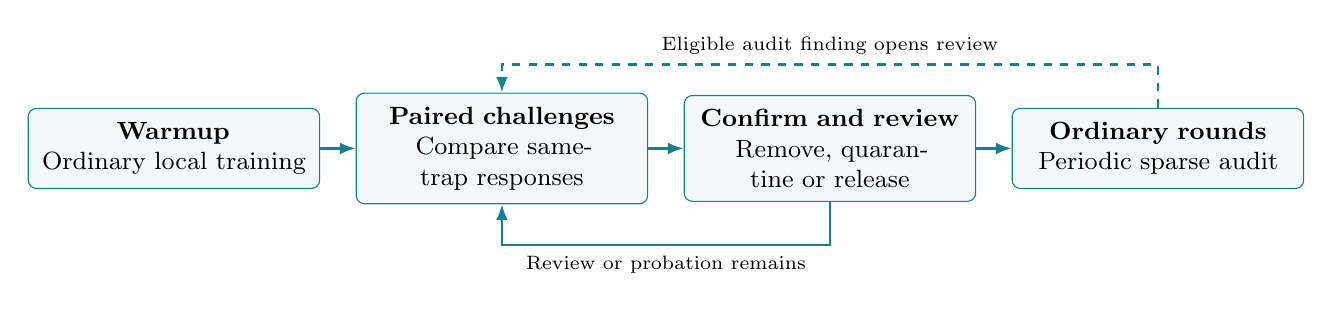
\begin{tikzpicture}[font=\small,
 box/.style={draw=baitteal,fill=baitteal!5,rounded corners=3pt,
 text width=3.35cm,minimum height=1.0cm,align=center,inner sep=5pt},
 arrow/.style={-{Latex[length=2mm]},thick,draw=baitteal}]
\node[box] (w) {\textbf{Warmup}\\Ordinary local training};
\node[box,right=0.45cm of w] (p) {\textbf{Paired challenges}\\Compare same-trap responses};
\node[box,right=0.45cm of p] (c) {\textbf{Confirm and review}\\Remove, quarantine or release};
\node[box,right=0.45cm of c] (s) {\textbf{Ordinary rounds}\\Periodic sparse audit};
\draw[arrow] (w)--(p);\draw[arrow] (p)--(c);\draw[arrow] (c)--(s);
\draw[arrow] (c.south)--++(0,-0.55)-| node[pos=.25,below,font=\scriptsize]{Review or probation remains} (p.south);
\draw[arrow,dashed] (s.north)--++(0,0.55)-| node[pos=.25,above,font=\scriptsize]{Eligible audit finding opens review} (p.north);
\end{tikzpicture}
\caption{BaitFL workflow.}\label{fig:short-flow}
\end{figure*}

\subsection{Challenges and Response Summaries}
After ten warmup rounds, each ten-round paired cycle freezes the current
global model $w^{(c)}$ and constructs independent traps $A$ and $B$.
For floating tensor $k$,
\begin{equation}
\tau_{a,k}=w^{(c)}_k+0.01\max\{\operatorname{sd}(w^{(c)}_k),10^{-4}\}\xi_{a,k},
\end{equation}
where $a\in\{A,B\}$ and $\xi_{a,k}\sim\mathcal N(0,I)$ independently.
Both traps remain fixed throughout the cycle. Floating buffers are
included and integer counters are unchanged.

Initially, clients are shuffled into at most ten groups, and each client
receives each trap once. In later cycles, clients under review alternate
between traps, while the remaining clients receive each trap once.
For each client and trap, one response position is selected uniformly
before responses are observed. Only those selected summaries enter the
cycle decision, preventing retrospective selection of unusual responses.
Incomplete paired coverage cannot authorize removal.

For each selected update $\Delta_i^a$, the server records its norm
$r_i^a=\|\Delta_i^a\|_2$ and normalized tensor profile
\begin{equation}
p^a_{i,k}=\frac{\|\Delta^a_{i,k}\|_2}{\sum_j\|\Delta^a_{i,j}\|_2}.
\end{equation}
The profile is zero if the denominator is below $10^{-6}$. It describes
how update magnitude is distributed across tensors. Each client is
compared with the other active clients receiving the same trap, including
quarantined and unresolved peers. Let $m_i^a,d_i^a$ be the median and
median absolute deviation (MAD) of peer norms. For profile distance
$\rho_i^a=\|p_i^a-\widetilde p_{-i}^a\|_2$, the reference
$\widetilde p_{-i}^a$ is the coordinatewise peer median. Peer distances
to that reference have median $\mu_i^a$ and MAD $\delta_i^a$. Scores are
\begin{equation}
z_i^{n,a}=\frac{r_i^a-m_i^a}{d_i^a/\Phi^{-1}(0.75)},\qquad
z_i^{p,a}=\frac{\rho_i^a-\mu_i^a}{\delta_i^a/\Phi^{-1}(0.75)}.
\end{equation}
Here $\Phi$ is the standard normal cumulative distribution function.
Missing comparisons or zero MAD leave the score undefined. Exact
send-back is checked separately through a zero update norm or a model
fingerprint matching the immediately previous model sent to that client.

\subsection{Screening and Geometric Certification}
Screening uses $D_i^a=z_i^{p,a}-z_i^{n,a}$ for each trap and their average.
Each view has $\lceil\sqrt{n_v}\rceil$ histogram bins, where $n_v$ is the
number of valid paired observations. Otsu splitting nominates a minority
above the boundary~\cite{otsu1979threshold}. The lower side of the
average-view split must contain a majority of all active clients.
Joint client resampling across the three views gives 99\% split intervals
from 1,000 bootstrap replicates~\cite{efron1979bootstrap}. Scores above
every upper boundary nominate suspicion, those below every lower
boundary are clear, and the rest are unresolved. If a reliable split is
unavailable, negative norm scores on both traps nominate suspicion.
Neither negative is clear, and mixed or undefined scores are unresolved.
The bootstrap intervals measure split stability, not false-removal risk.

A nomination alone cannot certify removal. Let $\mathcal U$ be the
nominated cohort and $\mathcal V$ the remaining active population.
With $n$ active clients, statistical evidence requires
\begin{equation}
\left\lceil\frac{n}{\lceil\sqrt n\rceil}\right\rceil
\leq |\mathcal U|<|\mathcal V|.
\end{equation}
For a given raw signal, let $Q_q$ denote an empirical quantile and
$I_U=Q_{.75}(\mathcal U)-Q_{.25}(\mathcal U)$. A low-norm certificate
requires both
\begin{equation}
\begin{split}
Q_{.25}(\mathcal V)-Q_{.75}(\mathcal U)&>I_U,\\
\min(\mathcal V)-Q_{.75}(\mathcal U)&>I_U,
\end{split}
\end{equation}
and an individual norm below the peer median. For high profile distances,
write $I_V$ for the peer IQR and
$g=Q_{.25}(\mathcal U)-Q_{.75}(\mathcal V)$. Require $g>I_U$, $g>0$,
and either
\begin{equation}
Q_{.25}(\mathcal U)-\max(\mathcal V)>I_U
\quad\text{or}\quad
\frac{I_U}{|\mathcal U|-1}<\frac{I_V}{|\mathcal V|-1}.
\end{equation}
The individual profile distance must also exceed the peer median.
Undefined measurements and insufficient support cannot certify a client.
The profile rule permits a concentrated cohort after an interquartile
gap, so persistent honest outliers can still pass it. These are geometric
heuristics, not calibrated hypothesis tests.

\subsection{Confirmation, Review and Rehabilitation}
The same component must certify a client on both traps for a
\emph{strong} cycle outcome. An uncertified nomination is
\emph{unresolved} and does not automatically trigger quarantine.
Separate norm and profile counters increment once per fresh complete
cycle. Statistical removal requires a fresh certificate that raises its
own component count to two. The cycles need not be consecutive, but
norm and profile counts never combine. Ambiguity preserves them and two
consecutive clear cycles reset them. Exact send-back instead requires
paired evidence in two consecutive complete cycles. Earliest removal
under the study schedule is round 30.

Strong evidence starts quarantine and a two-cycle review budget. Fresh
strong evidence renews it, while other completed cycles consume it.
Expiry releases an unconfirmed client even if evidence remains in memory.
Two consecutive clear outcomes rehabilitate a client, followed by one
additional clear probation cycle. Unconfirmed release starts a cooldown
of two sparse audits. Weak flags cannot renew exclusion. An unresolved
client may contribute ordinary responses whenever it is not quarantined.

\begin{algorithm}[t]
\caption{BaitFL training and auditing}\label{alg:short-overall}
\begin{algorithmic}[1]\small
\State Initialize records, component counts and quiet clock $\sigma=\bot$
\State Run ten ordinary warmup rounds
\State Schedule initial paired coverage
\While{the training horizon is not reached}
 \If{initial coverage, review or probation is active}
  \State Create two fixed traps and preselect response positions
  \State Run up to ten paired-cycle rounds, deferring final aggregation
  \If{paired coverage is complete}
   \State Screen peers and certify each component on both traps
   \State Update separate counts and consecutive send-back streaks
   \State Remove only on fresh confirmed evidence
   \State Apply quarantine, review expiry and rehabilitation
   \State $\sigma\gets$ current round if review/probation is empty, else $\bot$
  \EndIf
  \State Finish aggregation using the updated eligible set
 \ElsIf{$\sigma\ne\bot$ and ten quiet rounds have passed}
  \State Send one fresh trap to all active clients
  \State $\mathcal F\gets$ single-trap findings
  \State Open review for findings outside cooldown, without quarantine
  \State Decrease cooldown counters
  \State $\sigma\gets$ current round if $\mathcal F=\emptyset$, else $\bot$
 \Else
  \State Run one ordinary round and aggregate eligible responses
 \EndIf
\EndWhile
\end{algorithmic}
\end{algorithm}

\subsection{Sparse Audits and Aggregation}
When review and probation are empty, ordinary training continues with
an audit after ten quiet rounds. One fresh trap goes to all active
clients. A single-trap certificate or exact send-back opens two cycles
of review only if the client is outside cooldown. It cannot update
statistical counts, quarantine immediately or authorize removal.

The implemented quiet clock restarts only when the raw finding set
$\mathcal F$ is empty, as shown in Algorithm~\ref{alg:short-overall}.
If all nonempty findings are blocked by cooldown, review remains empty
and the unset clock can prevent subsequent audits. This pattern occurs
in none of the 622 recorded audits. An eligible-set clock guard agrees
on those traces but has not been used to recompute the results.

Let $\mathcal A_t$ contain ordinary-model recipients that are not
quarantined or newly removed. Eligible updates receive equal weights:
\begin{equation}
w_{t+1}=w_t+\frac{1}{|\mathcal A_t|}\sum_{i\in\mathcal A_t}\Delta_{t,i}.
\end{equation}
An empty set leaves the model unchanged. Trap responses never enter
aggregation, and trap training replaces ordinary local training for that
round. BaitFL and the no-defense comparison use the same client weighting.
Settings are fixed across the reported grid rather than tuned separately
for individual attacks or partitions.

\section{Experimental Evaluation}\label{sec:results-short}
\subsection{Setup and Reporting}
The study uses MNIST and CIFAR-10~\cite{lecun1998gradient,krizhevsky2009learning},
IID and Dirichlet non-IID partitions with $\alpha=0.5$, all four
strategies, and 30\% and 40\% free riders. Each configuration has
multi-seed evaluation. Federations contain 100 clients and run for
100 rounds. Honest clients train for three local SGD epochs with learning
rate 0.01, momentum 0.9 and batch size 32. FR3 uses $H=5$.

MNIST uses convolutional blocks with 16 and 32 channels and a 128-unit
hidden classifier. CIFAR-10 uses 32, 64 and 128 channels with BatchNorm
and a 256-unit classifier. Images are normalized without augmentation.
Execution is on CPU with six PyTorch threads. Independent random streams
control partitioning, identities, initialization, training and audits.

Detection rates count permanent removals, excluding temporary quarantine
and unresolved status. Table~\ref{tab:performance} pools counts across
attacks and seeds within each setting. Accuracy is the mean and sample
standard deviation across seeds for each attack. Runs are the experimental
units, since clients share a training trajectory. Pooled precision
describes observed outcomes rather than uncertainty from independent
client trials. Honest-response withholding counts trap and quarantine
client-rounds once, relative to active honest client-rounds.

\input{generated/performance.tex}

\subsection{Detection and Honest-Client Impact}
All 3,360 evaluated free riders are removed, with no false negatives.
Three honest clients are removed among 6,240 honest client-cases,
concentrated in two runs. Most executions finish detection at round 30,
while the slowest reaches round 90. FR1 and FR2 are consistently removed
at the earliest opportunity. The delayed cases involve history-based
responses. Table~\ref{tab:performance} shows final mean accuracy between
98.83\% and 99.02\% on MNIST and between 74.51\% and 77.84\% on CIFAR-10.

All honest removals occur in MNIST non-IID at 40\%. Two clients under
FR3 receive repeated profile certificates and are removed at round 30.
One under FR4 receives norm certificates in separated cycles and is
removed at round 90. This setting has 480 correct and three incorrect
removals, giving $480/483=99.38\%$ pooled precision. Repeated challenges
can reinforce an error when legitimate data heterogeneity persistently
resembles the geometric evidence used by the detector.

Temporary costs extend beyond those three errors. There are 32 honest
client-cases with quarantine, totaling 620 client-rounds, although none
remains quarantined at completion. Even IID cases with no honest removal
or quarantine withhold roughly 11\% of honest responses through the trap
schedule. Non-IID FR3 at 40\% withholds 12.86\% on MNIST and 17.08\% on
CIFAR-10. These are lost contributions, regardless of server computation.

Unresolved status is also common after free riders have gone. The same
non-IID FR3 setting ends with means of 37 unresolved honest clients on
MNIST and 43 on CIFAR-10, out of 60 honest clients. The label alone
does not prevent ordinary aggregation or renew quarantine. It records
remaining evidence and is not a reliable final free-rider classification
in these settings.

\subsection{Utility Relative to No Defense}
Completed seed-matched no-defense runs use the same partitions, training
and equal-weight aggregation. Across available pairs, BaitFL's final
accuracy differs by a mean of $+0.10$ percentage points on MNIST and
$+0.60$ on CIFAR-10. These descriptive averages indicate comparable or
slightly higher accuracy, rather than a consistent improvement in every
setting. Baseline replication coverage is uneven across datasets.

Saved trajectories also permit illustrative time-to-target comparisons
at 98\% MNIST and 70\% CIFAR-10 accuracy. Averaging seeds within each
attack and then attacks equally, MNIST non-IID at 40\% reaches the target
in 16.48 minutes with BaitFL and 23.28 minutes without defense. The
corresponding CIFAR-10 means are 48.02 and 58.32 minutes. Targets were
chosen after examining the trajectories. These observations combine the
benefit of removing free riders with the cost of withheld contributions.
They do not isolate auditing overhead or establish a controlled timing
advantage. An honest-only oracle and matched execution clocks are needed
to separate these effects.

\subsection{Instrumented Computation Cost}
Separate 100-round executions compare BaitFL and a reimplementation of
STD-DAGMM on non-IID FR3 at 40\%, using the same client count, local
epochs and CPU-thread setting. STD-DAGMM retains all clients and freshly
fits an auxiliary model for five epochs per round. This fitting budget
is a reproduction choice, not an author-specified schedule or evidence
of convergence~\cite{lin2019freeriders,zong2018dagmm}.

\begin{table}[t]
\centering\footnotesize\setlength{\tabcolsep}{4pt}
\caption{Mean computation time per round (seconds).}\label{tab:short-timing}
\begin{tabular}{lrrrr}\toprule
\multirow{2}{*}{Stage}&\multicolumn{2}{c}{MNIST}&\multicolumn{2}{c}{CIFAR-10}\\
\cmidrule(lr){2-3}\cmidrule(lr){4-5}
&BaitFL&STD&BaitFL&STD\\\midrule
Traps and scheduling&0.0018&0&0.018&0\\
Features/preparation&0.198&0.045&0.729&0.115\\
Auxiliary fitting&0&15.76&0&42.09\\
Scoring and decisions&0.016&0.335&0.043&0.827\\\midrule
Checking subtotal&0.215&16.14&0.791&43.03\\
All computation&36.92&52.26&88.56&120.05\\\bottomrule
\end{tabular}
\end{table}

Table~\ref{tab:short-timing} separates the checking stages, whose
subtotals are included in total computation. BaitFL checking averages
0.215 seconds per round on MNIST and 0.791 on CIFAR-10, respectively
0.58\% and 0.89\% of total computation including local training and
global evaluation. These shares are not incremental overhead against
no defense. STD-DAGMM fitting averages 15.76 and 42.09 seconds per round.
Figure~\ref{fig:short-timing} shows the corresponding checking and total
computation times. Overall computation is 29.35\% lower on MNIST and
26.23\% lower on CIFAR-10 in these particular executions.

\begin{figure}[t]
\centering
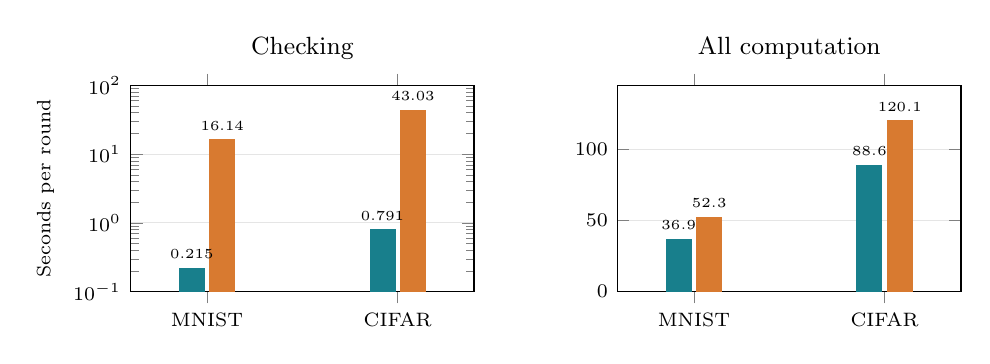
\begin{tikzpicture}
\begin{axis}[width=.49\columnwidth,height=4.2cm,
 ybar,bar width=9pt,ymode=log,log origin=infty,ymin=.1,ymax=100,
 symbolic x coords={MNIST,CIFAR},xtick=data,
 ylabel={Seconds per round},title={Checking},
 title style={font=\small},tick label style={font=\scriptsize},
 label style={font=\scriptsize},enlarge x limits=.4,
 point meta=explicit symbolic,
 nodes near coords,nodes near coords style={font=\tiny},
 ymajorgrids,grid style={gray!20}]
\addplot[fill=baitteal,draw=baitteal] coordinates {(MNIST,.215)[0.215](CIFAR,.791)[0.791]};
\addplot[fill=stdorange,draw=stdorange] coordinates {(MNIST,16.14)[16.14](CIFAR,43.03)[43.03]};
\end{axis}
\begin{axis}[at={(.51\columnwidth,0)},anchor=south west,
 width=.49\columnwidth,height=4.2cm,ybar,bar width=9pt,ymin=0,ymax=145,
 symbolic x coords={MNIST,CIFAR},xtick=data,title={All computation},
 title style={font=\small},tick label style={font=\scriptsize},
 enlarge x limits=.4,nodes near coords,
 nodes near coords style={font=\tiny,/pgf/number format/fixed,/pgf/number format/precision=1},
 ymajorgrids,grid style={gray!20}]
\addplot[fill=baitteal,draw=baitteal] coordinates {(MNIST,36.92)(CIFAR,88.56)};
\addplot[fill=stdorange,draw=stdorange] coordinates {(MNIST,52.26)(CIFAR,120.05)};
\end{axis}
\end{tikzpicture}
\par\smallskip{\footnotesize\textcolor{baitteal}{\rule{8pt}{6pt}} BaitFL\quad
\textcolor{stdorange}{\rule{8pt}{6pt}} STD-DAGMM}
\caption{Instrumented round times. BaitFL is the left bar of each pair.
The checking panel uses a logarithmic scale.}\label{fig:short-timing}
\end{figure}

The comparison measures two native workflows with different participation
and runtime behavior. It does not rank detection effectiveness. The stored
five-epoch STD-DAGMM flags identify none of the 4,000 free-rider responses
in either execution, while flagging 2,200 honest responses on MNIST and
2,196 on CIFAR-10. These single-configuration roundwise flags are not
matched to BaitFL's permanent-removal endpoint. A comparative detection
benchmark requires validated baseline settings and common endpoints.
Network transmission and device energy are not measured.

\section{Complexity and Limitations}
Let $P$ be floating model coordinates, $L$ floating tensors, $N$ active
clients, $B$ bootstrap replicates and $K=\lceil\sqrt N\rceil$ histogram
bins. Response features require $O(NP)$ work per round. Current
leave-one-out comparisons cost $O(N^2(L+\log N))$ per decision, while
bootstrap splitting costs $O(B(N+K))$. For $T$ rounds, $M$ paired cycles
and $A$ sparse audits, total detector work is bounded by
\begin{equation}
\begin{split}
O\bigl(TNP+(M+A)\bigl[N^2(L+\log N)\\
{}+B(N+K)\bigr]\bigr).
\end{split}
\end{equation}
Working state is $O(P+NL+BN+BK)$, excluding ordinary training and
research logs. Shared challenges and compact summaries avoid an auxiliary
neural detector, but peer comparisons remain quadratic in population.
The lightweight claim is therefore supported at 100 clients rather than
established for arbitrarily large federations.

Challenges replace ordinary models in the existing exchange, preserving
the nominal $O(NP)$ model-payload order per round. They still consume
local training rounds whose outputs are withheld. Low server checking
cost cannot establish low utility, network or energy cost.

The threat model excludes collusion, intermittent training and adaptive
trap recognition. An attacker that recognizes a challenge or reproduces
its response statistics may evade the detector. Honest non-IID clients
can also produce persistent outliers, as the observed removals show.
Two-trap and cross-cycle confirmation reduce reliance on an isolated
observation but cannot resolve this fundamental ambiguity. Individual
response visibility excludes conventional secure aggregation, and the
fixed population does not test dropout or client sampling.

Experiments cover two datasets, two relatively high attacker shares and
four specified non-adaptive strategies. They do not reproduce every
published stochastic or convergence-aware attack. Detector settings were
fixed after development without a separate held-out tuning study.
Priorities for further evaluation include honest-only and low-prevalence
conditions, passive-detector ablations, validated comparative detection,
and controlled oracle timing. The cooldown-clock edge case also requires
corrected-code reruns before broader implementation claims.

\section{Conclusion}
BaitFL uses hidden model challenges, compact response features and
repeated confirmation to detect persistent free riding without an
auxiliary learned detector. All tested free riders are removed, with
three honest removals concentrated in non-IID runs. Instrumented checking
cost is small at 100 clients, while withheld honest contributions and
persistent statistical ambiguity remain practical costs. The results
support lightweight server computation under the stated threat model
and motivate further tests of honest-only operation, lower attacker
shares and adaptive behavior.

% Balance the final columns using IEEEtran's bibliography break.
\IEEEtriggeratref{7}
\bibliographystyle{IEEEtran}
\bibliography{refs}
\end{document}
